\documentclass[11pt]{article}

\usepackage[review]{acl}
\usepackage{times}
\usepackage{latexsym}
\usepackage[T1]{fontenc}
\usepackage[utf8]{inputenc}
\usepackage{kotex}
\usepackage{microtype}
\usepackage{inconsolata}
\usepackage{graphicx}
\usepackage{booktabs}
\usepackage{multirow}
\usepackage{amsmath}
\usepackage{amssymb}
\usepackage{tabularx}
\usepackage{tikz}
\usetikzlibrary{arrows.meta,positioning,fit,calc}

\definecolor{shortblue}{RGB}{225,238,249}
\definecolor{longorange}{RGB}{252,232,210}
\definecolor{stagegreen}{RGB}{226,242,230}
\definecolor{stagegray}{RGB}{242,242,242}

\title{웹페이지는 얼마나 자세히 말해야 하는가?\\
웹 GUI 사전학습에서 서술 상세도에 관한 통제 연구}

\author{Anonymous ACL submission}

\begin{document}
\maketitle

\begin{abstract}
시각 기반 웹 에이전트는 일반적으로 웹페이지 지각 사전학습,
명령어 튜닝, 행동 궤적 학습의 여러 단계를 거친다. 그러나 첫 단계에
대해서는 정립된 학습 레시피가 없으며, 웹페이지를 텍스트로 얼마나
자세히 설명해야 하는지도 충분히 연구되지 않았다. 본 연구는 웹 GUI
사전학습에서 서술 상세도의 효과를 통제된 조건에서 분석한다. 동일한
15만 장의 데스크톱 웹 스크린샷과 공통 구조화 사실로부터 평균
110단어의 짧고 상호작용 중심적인 설명과 평균 3,656자의 포괄적인
설명을 합성한다. 각 설명 집합을 동일한 123만 개의 요소 그라운딩
예제와 혼합하여 9B 시각언어모델을 전체 파인튜닝한다. 이후 세 조건에
동일한 10만 개의 명령어 데이터와 10만 개의 행동 궤적을 순차적으로
학습하고, 각 단계의 체크포인트를 웹페이지 이해, 그라운딩, 텍스트
밀집 시각 이해 전이, 웹 에이전트 벤치마크에서 평가한다. 이 설계는
포괄적 설명이 사전학습 직후 유리한지를 넘어 그 효과가 후속
과제특화 학습 이후에도 유지되는지를 검증한다. 현재 주요 학습과
평가는 진행 중이며, 본 논문은 비교 조건, 합성 데이터 검증 절차,
단계별 평가 프로토콜을 제시한다.
\end{abstract}

\section{서론}

웹 그래픽 사용자 인터페이스(GUI)는 텍스트, 레이아웃, 현재 상태,
가능한 행동을 동시에 해석해야 하는 고밀도 시각 환경이다. 최근에는
DOM과 규칙 기반 도구에 의존하는 에이전트에서 벗어나, 스크린샷을
직접 보고 브라우저 행동을 예측하는 시각언어 에이전트가 활발히
연구되고 있다 \citep{qin2025uitars,gupta2026molmoweb}. 한편
VisualWebBench는 현재 멀티모달 모델이 웹페이지 OCR, 세부 이해,
그라운딩에서 여전히 큰 성능 격차를 보인다는 점을 드러냈다
\citep{liu2024visualwebbench}. 대규모 웹 UI 명령어 데이터가 웹
과제뿐 아니라 문서와 차트 등 비웹 텍스트 밀집 과제에도 전이된다는
결과 \citep{liu2025multiui}는 웹페이지 supervision이 범용적인 시각
표현을 학습하는 데 유용할 가능성을 보여준다.

그러나 기존 웹 GUI 모델은 데이터 출처, 과제 혼합 비율, 행동 공간,
학습 단계가 서로 달라 무엇이 최종 성능을 만드는지 분리하기 어렵다.
특히 새로운 기반 모델에서 웹 GUI 학습을 시작할 때
\emph{명령 수행이나 행동 궤적을 배우기 전에 웹페이지로부터 무엇을
학습시켜야 하는가}라는 기본 질문에 명확한 답이 없다. LLaVA 계열과
같은 범용 멀티모달 모델은 이미지--텍스트 정렬 또는 시각 명령어
튜닝을 먼저 수행한다 \citep{liu2023llava,liu2024llavanext}. 웹 GUI
모델도 지각 및 그라운딩 데이터를 사용하지만, 화면 설명의 적절한
상세도는 분명하지 않다.

짧은 설명은 페이지의 목적, 핵심 상태, 대표 상호작용에 supervision을
집중한다. 반대로 긴 설명은 작은 텍스트와 상태, 표의 각 항목,
행동 가능한 요소까지 보존하여 더 풍부한 웹 표현을 만들 수 있다.
그러나 장문은 중요도가 낮은 요소의 나열에 모델 용량을 소비하거나,
후속 명령어 및 궤적 학습에서 그 효과가 사라질 수도 있다. 그림
\ref{fig:contrast}는 본 연구의 두 supervision 조건과 공통으로
통제되는 요소를 요약한다.

\begin{figure}[t]
\centering
\begin{tikzpicture}[
  font=\footnotesize,
  box/.style={draw, rounded corners=2pt, align=center,
              minimum height=8mm, inner sep=2.5pt},
  arrow/.style={-{Latex[length=1.8mm]}, thick},
  note/.style={font=\scriptsize, align=center}
]
\node[box, fill=stagegray, text width=.78\columnwidth] (screen)
  {\textbf{동일한 웹 화면과 Stage 1 evidence}\\
   content · state · relation · affordance · coordinate};
\node[box, fill=shortblue, below=7mm of screen,
      xshift=-.27\columnwidth, text width=.25\columnwidth] (concise)
  {\textbf{Concise}\\salient evidence};
\node[box, fill=stagegreen, below=7mm of screen,
      text width=.25\columnwidth] (balanced)
  {\textbf{Balanced}\\section-level\\evidence};
\node[box, fill=longorange, below=7mm of screen,
      xshift=.27\columnwidth, text width=.25\columnwidth] (comprehensive)
  {\textbf{Compre-}\\\textbf{hensive}\\near-complete\\evidence};
\node[box, fill=stagegray, below=10mm of balanced,
      text width=.78\columnwidth] (eval)
  {\textbf{공통 grounding 및 후속 학습}\\
   coverage 분석 · targeted diagnostic\\공개 benchmark · agent transfer};
\draw[arrow] (screen.south) -- (concise.north);
\draw[arrow] (screen.south) -- (balanced.north);
\draw[arrow] (screen.south) -- (comprehensive.north);
\draw[arrow] (concise.south) -- (eval.north west);
\draw[arrow] (balanced.south) -- (eval.north);
\draw[arrow] (comprehensive.south) -- (eval.north east);
\end{tikzpicture}
\caption{\textbf{웹페이지 verbalization의 정보 포괄성 비교.}
동일한 화면과 Stage 1 evidence를 서로 다른 information budget으로
언어화한다. 세 recipe는 평균 coverage가 증가하지만 sample별
evidence 집합의 엄격한 포함관계를 가정하지 않는다. Grounding
데이터와 후속 학습은 동일하게 유지한다.}
\label{fig:contrast}
\end{figure}


본 연구는 \textbf{간결한 설명(Concise)}과 \textbf{포괄적
설명(Comprehensive)}을 비교한다. 두 조건은 스크린샷, 1단계 구조화
사실, 좌표 규약, 외부 그라운딩 데이터, 기반 모델, 최적화 설정,
후속 데이터를 공유한다. 바뀌는 것은 설명의 길이와 이에 수반되는
정보 선택뿐이다. 효과는 사전학습(PT) 직후, 공통 명령어 튜닝(IT)
직후, 행동 궤적 지도학습(Traj) 직후의 세 지점에서 측정한다.

본 연구의 기여는 다음과 같다.
\begin{itemize}
    \item 그라운딩 양과 후속 데이터를 고정한 상태에서 웹 GUI
    사전학습의 서술 상세도를 비교하는 통제 실험을 설계한다.
    \item 아홉 개 체크포인트를 통해 PT의 효과가 어느 단계에서
    나타나고 후속 학습 이후까지 유지되는지 추적한다.
    \item 접근성 트리의 bounding box 좌표를 teacher가 추정하지 않고
    인용하도록 하며, 프로그램 검증으로 좌표 발명을 제거하는 2단계
    합성 파이프라인을 제시한다.
\end{itemize}
현재 주요 평가가 진행 중이므로 어느 조건이 우월하다고 미리
주장하지 않고, 기여를 연구 질문과 방법론 중심으로 기술한다.

\section{관련 연구}

\paragraph{멀티모달 사전학습과 명령어 튜닝.}
LLaVA는 시각 인코더와 언어모델을 간단한 projection으로 연결하고
합성 시각 명령어 데이터로 학습하는 효과적인 방식을 보였다
\citep{liu2023llava}. LLaVA-1.5는 동일 계열의 구조에서 데이터와
학습 설정을 개선하여 강한 기준선을 제시하였다
\citep{liu2024llavanext}. 이 연구들은 시각--언어 정렬과 후속 명령어
튜닝을 구분할 필요성을 보여준다. 본 연구는 이 문제를 웹 도메인으로
좁혀, 동일 파이프라인 안에서 화면마다 언어화되는 정보량만을
변화시킨다.

\paragraph{웹페이지 이해 및 GUI 에이전트.}
VisualWebBench는 OCR, 캡셔닝, 질의응답, 행동 예측, 그라운딩을
포함하는 일곱 가지 웹페이지 과제를 평가한다
\citep{liu2024visualwebbench}. MultiUI는 백만 개의 웹페이지 UI에서
730만 개의 멀티모달 명령어 예제를 구축하고, 문서ㆍ차트ㆍGUIㆍ에이전트
과제로의 전이를 보고하였다 \citep{liu2025multiui}. UI-TARS는 대규모
GUI 지각 데이터, 통합 행동 표현, 상호작용 궤적을 이용해
스크린샷 기반 native GUI agent를 학습한다 \citep{qin2025uitars}.
MolmoWeb 역시 GUI 지각 데이터와 10만 개 이상의 합성 궤적, 3만 개
이상의 인간 시연을 결합한다 \citep{gupta2026molmoweb}. 이들은 행동
학습 이전 또는 행동 학습과 함께 지각 supervision이 필요함을
보이지만, 다른 조건을 맞춘 상태에서 설명의 상세도를 직접
비교하지는 않는다.

\section{통제된 데이터 구축}

\subsection{원본 스크린샷과 좌표}

WebUI-350K에서 Tranco 도메인 순위, 도메인별 상한, 라운드로빈
선별을 이용해 영어 데스크톱 스크린샷 150,000장을 선택한다. 각
예제는 $1920\times1080$ viewport slice이다. Chrome 접근성 트리에서
요소의 역할, 이름, 클릭 가능 여부, bounding box를 얻는다. 이미지
너비와 높이가 각각 $W,H$이고 bounding box가 $(x,y,w,h)$일 때
중심점을 다음과 같이 공통 정수 좌표계로 변환한다.
\begin{equation}
\hat{x}=\operatorname{clip}\!\left(
\operatorname{round}\left(\frac{x+w/2}{W}\times999\right),0,999\right),
\end{equation}
$\hat{y}$도 같은 방식으로 계산한다. 합성 모델은 계산된 좌표를
프롬프트로 전달받아 그대로 인용하며, 픽셀만 보고 좌표를 추정하지
않는다.

\subsection{공통 사실 추출}

Qwen3.5-397B-A17B teacher를 이용한 2단계 파이프라인을 구성한다.
Stage 1은 스크린샷과 화면에 보이는 접근성 트리 요소를 입력받아
페이지 유형, 팝업 상태, 가시 텍스트 사실, 현재 행동 가능한 요소를
구조화한다. 각 affordance는 이름, 행동 유형, 예상 결과, 좌표를
포함한다. 총 148,187개의 유효한 사실 레코드를 얻었으며 두 설명
조건 모두 이 파일을 공유한다. 따라서 조건 간 차이는 teacher가
서로 다른 사실을 추출했기 때문이 아니라, 같은 사실을 어떤
상세도로 언어화했기 때문에 발생한다.

\subsection{간결한 설명과 포괄적 설명}

\paragraph{포괄적 설명.}
Long prompt는 제공된 모든 가시 사실과 affordance를 하나의
자기완결적 장문에 포함하도록 요구한다. 표의 행과 열, 요소 좌표를
보존하고, 관찰된 사실과 아직 실행하지 않은 행동의 예상 결과를
구분한다. 이미지 해시에 따라 전개 순서와 문체를 결정론적으로
변주한다. 반복 퇴화가 발생한 25건을 제거한 뒤 147,967개의 설명을
얻었으며 평균 길이는 3,656자이다.

\paragraph{간결한 설명.}
Short prompt는 3--5문장, 약 90--130단어로 페이지 유형, 주된 목적,
가장 중요한 가시 상태, 최대 두 개의 핵심 상호작용 목표를
서술하도록 한다. 출력에 행동 요소가 등장하면 제공된 좌표를 반드시
함께 보존한다. 따라서 Long 조건이 정보를 열거한다면 Short 조건은
정보를 선택하고 압축한다. 최종 데이터는 143,097건이며 평균
110.2단어, 4.24문장이다.

\begin{table}[t]
\centering
\small
\setlength{\tabcolsep}{5pt}
\begin{tabular}{lrr}
\toprule
 & Short & Long \\
\midrule
화면 설명 & 143K & 148K \\
공통 그라운딩 & 1.2M & 1.2M \\
전체 PT 예제 & 1.37M & 1.38M \\
\bottomrule
\end{tabular}
\caption{\textbf{사전학습 데이터 구성.} 두 조건은 같은 그라운딩
데이터와 좌표계를 공유한다. 표는 전체 구축 규모이며, 통제 비교는
두 설명이 모두 유효한 동일 화면의 교집합에서 수행한다.}
\label{tab:data}
\end{table}


\paragraph{프로그램 기반 검증.}
모든 Short 생성 결과의 좌표를 Stage-1 좌표 집합과 대조한다.
148,187개 입력 가운데 두 차례 재시도 후에도 4,896건이 규칙을
위반하였다. 이 중 4,671건은 존재하지 않는 좌표를 생성했고,
194건은 문장 수, 31건은 단어 수 제약을 어겼다. 최종 집합에는 총
392,055개의 좌표 언급(예제당 평균 2.74개)이 있으며 검출된 좌표
발명은 0건이다. 이 결과는 합성 데이터의 구조적 제약을 프롬프트에만
맡기지 않고 검증기로 강제해야 함을 보여준다.

\subsection{동일한 그라운딩 혼합}

각 설명 집합을 동일한 1,228,336개의 영어 UGround 예제와 혼합한다.
UGround는 요소 설명을 동일한 0--1000 좌표계의 한 점에 대응시킨다.
두 혼합 데이터는 seed 42와 동일한
\texttt{prompt}/\texttt{completion}/\texttt{images} 스키마를 사용한다.
그라운딩이 두 PT 데이터의 약 90\%를 차지하므로, Long 조건이
설명에서 더 많은 좌표를 포함한다는 이유만으로 별도의 그라운딩
예제를 더 받지는 않는다.

\section{학습 및 평가}

\subsection{학습 단계}

기반 모델은 Qwen3.5-9B이다. 모든 PT에서 전체 파라미터를 1 epoch
학습하며 bfloat16, cosine learning rate $10^{-5}$, warmup 3\%,
completion-only loss, 최대 길이 8192, effective batch size 256을
사용한다. 이미지는 최대 2,359,296 pixel로 입력하며 현재 해상도에서
3,009 image token에 해당한다. 모든 PT run에 gradient checkpointing을
적용한다.

PT 이후 Base, Short PT, Long PT 모델은 같은 순서의 100K IT 예제를
학습한다. 이 데이터는 MolmoWeb SyntheticQA 70K와 필터링한
LLaVA-NeXT 30K로 구성한다. 후속 일반화 평가와의 중복을 막기 위해
LLaVA-NeXT에서 DocVQA, ChartQA, DVQA, AI2D 출처를 제거한다. 세 IT
체크포인트에는 다시 동일한 99,999개의 trajectory 예제를 학습한다.
행동 공간은 \texttt{click}, \texttt{type}, \texttt{press},
\texttt{scroll}, \texttt{goto}, \texttt{go\_back}, \texttt{finish}의
일곱 가지로 통일한다.

\begin{figure*}[t]
\centering
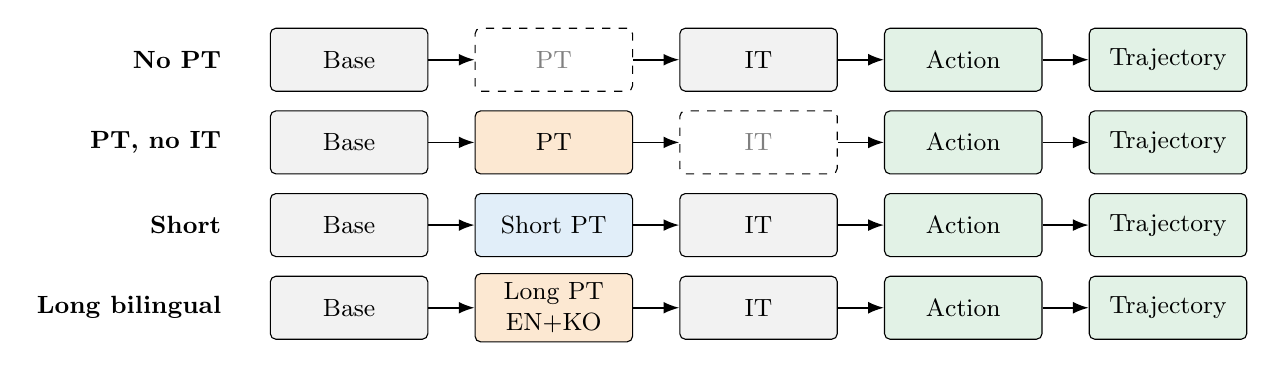
\begin{tikzpicture}[
  font=\small,
  stage/.style={draw, rounded corners=2pt, align=center,
                minimum width=20mm, minimum height=8mm},
  skip/.style={draw, rounded corners=2pt, align=center,
               minimum width=20mm, minimum height=8mm, dashed,
               text=gray},
  arrow/.style={-{Latex[length=2mm]}, semithick},
  row/.style={font=\small\bfseries, anchor=east}
]
\node[row] at (-0.5,0) {No PT};
\node[row] at (-0.5,-1.05) {PT, no IT};
\node[row] at (-0.5,-2.10) {Short};
\node[row] at (-0.5,-3.15) {Long bilingual};

\node[stage,fill=stagegray] (base0) at (1,0) {Base};
\node[stage,fill=stagegray] (base1) at (1,-1.05) {Base};
\node[stage,fill=stagegray] (base2) at (1,-2.10) {Base};
\node[stage,fill=stagegray] (base3) at (1,-3.15) {Base};

\node[skip]  (pt0) at (3.6,0) {PT};
\node[stage,fill=stagegray] (it0) at (6.2,0) {IT};
\node[stage,fill=stagegreen] (act0) at (8.8,0) {Action};
\node[stage,fill=stagegreen] (traj0) at (11.4,0) {Trajectory};

\node[stage,fill=longorange] (pt1) at (3.6,-1.05) {PT};
\node[skip]  (it1) at (6.2,-1.05) {IT};
\node[stage,fill=stagegreen] (act1) at (8.8,-1.05) {Action};
\node[stage,fill=stagegreen] (traj1) at (11.4,-1.05) {Trajectory};

\node[stage,fill=shortblue] (pt2) at (3.6,-2.10) {Short PT};
\node[stage,fill=stagegray] (it2) at (6.2,-2.10) {IT};
\node[stage,fill=stagegreen] (act2) at (8.8,-2.10) {Action};
\node[stage,fill=stagegreen] (traj2) at (11.4,-2.10) {Trajectory};

\node[stage,fill=longorange] (pt3) at (3.6,-3.15) {Long PT\\EN+KO};
\node[stage,fill=stagegray] (it3) at (6.2,-3.15) {IT};
\node[stage,fill=stagegreen] (act3) at (8.8,-3.15) {Action};
\node[stage,fill=stagegreen] (traj3) at (11.4,-3.15) {Trajectory};

\foreach \r in {0,1,2,3} {
  \draw[arrow] (base\r) -- (pt\r);
  \draw[arrow] (pt\r) -- (it\r);
  \draw[arrow] (it\r) -- (act\r);
  \draw[arrow] (act\r) -- (traj\r);
}
\end{tikzpicture}
\caption{\textbf{실제로 준비한 네 학습 경로.} 점선 상자는 해당
단계를 건너뜀을 뜻한다. 각 단계의 데이터 구성과 비교 목적은
본문에서 설명한다.}
\label{fig:pipeline}
\end{figure*}


그림 \ref{fig:pipeline}과 표 \ref{tab:checkpoints}는 전체 비교 구조를
보여준다. PT가 없는 분기는 PT 자체의 효과와 Short/Long 간 차이를
분리하는 기준선이다.

\begin{table}[t]
\centering
\small
\setlength{\tabcolsep}{3.5pt}
\begin{tabular}{clccc}
\toprule
ID & 체크포인트 & PT & IT & Traj \\
\midrule
C0 & Base & -- & -- & -- \\
C1 & Short PT & Short & -- & -- \\
C2 & Long PT & Long & -- & -- \\
C3 & Base + IT & -- & \checkmark & -- \\
C4 & Short PT + IT & Short & \checkmark & -- \\
C5 & Long PT + IT & Long & \checkmark & -- \\
C6 & Base + IT + Traj & -- & \checkmark & \checkmark \\
C7 & Short + IT + Traj & Short & \checkmark & \checkmark \\
C8 & Long + IT + Traj & Long & \checkmark & \checkmark \\
\bottomrule
\end{tabular}
\caption{\textbf{평가할 아홉 개 체크포인트.} 중간 체크포인트를
보존하여 PT 효과가 나타나는 지점과 후속 학습 이후의 유지 여부를
분리한다.}
\label{tab:checkpoints}
\end{table}


\subsection{연구 질문}

분석은 다음 세 질문을 중심으로 구성한다.
\textbf{RQ1:} Long PT는 PT 직후 웹페이지 이해 또는 그라운딩을
개선하는가?
\textbf{RQ2:} 두 조건의 차이는 공통 IT 이후에도 유지되는가, 아니면
과제특화 supervision에 의해 소거되는가?
\textbf{RQ3:} PT 서술 상세도는 최종 trajectory-following agent와
비웹 텍스트 밀집 이미지로의 전이에 영향을 미치는가?

\subsection{평가 벤치마크}

C0--C5는 VisualWebBench의 이해와 그라운딩을 분리하여 평가하고,
WebSRC, WebClick, ScreenSpot-v2, 한국어 웹 벤치마크를 함께
사용한다. DocVQA의 ANLS와 ChartQA의 relaxed accuracy로 비웹 텍스트
밀집 시각 이해 전이를 측정한다. C6--C8의 주요 에이전트 평가는
Multimodal-Mind2Web이며 cross-task, cross-website, cross-domain
분할을 각각 보고한다. 좌표 출력은 모든 평가에서 0--999 규약으로
해석한다.

\subsection{주요 결과 (진행 중)}

\begin{table*}[t]
\centering
\small
\begin{tabular}{lccccccc}
\toprule
& \multicolumn{3}{c}{Grounding} & \multicolumn{3}{c}{Web understanding} & \multicolumn{1}{c}{Gen.} \\
\cmidrule(lr){2-4}\cmidrule(lr){5-7}\cmidrule(lr){8-8}
Pretraining supervision & Screenspot$^{\dagger}$ & GroundUI$^{\dagger}$ & VisualWebBench-G & VWB-U & WebSRC & Korean Web & DocVQA \\
\midrule
Grounding-only & 70.83 & 69.90 & 50.19 & -- & -- & -- & -- \\
Info-L  & 81.92 & 76.00 & 68.99 & -- & -- & -- & -- \\
Info-M & 82.86 & 80.30 & 62.21 & -- & -- & -- & -- \\
Info-H & \textbf{83.25} & \textbf{80.60} & \textbf{75.78} & -- & -- & -- & -- \\
\bottomrule
\end{tabular}
\caption{\textbf{Description coverage에 따른 pretraining 결과.}
Info-L/M/H는 각각 $\bar\rho=0.13/0.44/0.98$의 description coverage 조건이다.
모든 조건은 동일한 스크린샷 집합과 grounding 데이터를 공유하며,
description coverage만 다르다. SS-v2는 ScreenSpot-v2,
VWB-G/U는 VisualWebBench의 grounding/understanding을 가리킨다.
$^{\dagger}$ mobile과 desktop split의 평균.}
\label{tab:main}
\end{table*}
\begin{table}[t]
\centering
\scriptsize
\setlength{\tabcolsep}{3pt}
\begin{tabularx}{\columnwidth}{@{}Xccc@{}}
\toprule
모델 & Task & Website & Domain \\
\midrule
Grounding-only & -- & -- & -- \\
Concise & -- & -- & -- \\
Balanced & -- & -- & -- \\
Comprehensive & -- & -- & -- \\
\bottomrule
\end{tabularx}
\caption{\textbf{동일한 post-training을 마친 네 조건의
Multimodal-Mind2Web 결과.} 열은 각각 cross-task, cross-website,
cross-domain 분할을 나타낸다.}
\label{tab:agent}
\end{table}


하나의 종합 점수만으로 결론을 선택하지 않는다. 예를 들어 Long
caption은 이해 성능에는 유리하지만 정밀 그라운딩에는 불리할 수
있고, PT 직후의 차이가 IT 이후 사라질 수도 있다. 따라서 C1--C2,
C4--C5, C7--C8을 각각 비교하고 C0, C3, C6으로 PT 자체의 한계
효과를 측정한다. 벤치마크가 허용하는 경우 paired bootstrap
confidence interval을 보고한다. 다만 학습 seed가 하나이므로 통계적
주장은 run 간 분산이 아니라 평가 표본의 불확실성으로 제한한다.

\section{논의}

본 연구의 ``설명 길이''는 순수한 출력 token 수 조작이 아니라
supervision 상세도의 대리변수이다. Short supervision은 중요 사실을
선택해야 하고 Long supervision은 추출된 사실과 행동을 거의 모두
보존한다. 따라서 과학적으로 비교되는 조건은 동일한 근거에서 만든
\emph{선택적 설명}과 \emph{포괄적 설명}이다.

Long PT의 이점이 Traj 이후에도 유지된다면, 행동 학습 전에 풍부한
지각 supervision을 구축할 근거가 된다. 반대로 IT 이후 차이가
사라진다면 비용이 큰 장문 합성이 최종 에이전트에 불필요할 수 있다.
Short PT가 우세하다면, 모든 요소를 빠짐없이 서술하는 목표가
중요도가 낮은 정보나 약하게 우선순위화된 학습 신호를 과도하게
제공했을 가능성을 검토해야 한다.

\section{한계}
\label{sec:limitations}

첫째, 두 caption의 화면 집합은 완전히 일치하지 않는다. 좌표 검증
과정에서 Short 예제가 4,870건 더 제거되었지만 전체 PT 행 수의
차이는 0.35\%이다. 더 엄밀한 후속 실험에서는 공통으로 통과한 화면
ID의 교집합만 사용해야 한다. 둘째, 현재 실험에서 설명 길이와 정보
선택 효과를 분리할 수 없다. 셋째, 모든 합성 설명이 하나의
teacher에서 생성되어 teacher 편향이 두 조건에 공통으로 존재한다.
넷째, 학습은 1 epoch와 단일 seed로 수행되어 run 간 분산을 추정하지
못한다. 다섯째, Traj 단계의 이미지 pixel 상한이 PT보다 낮고,
\texttt{go\_back} 정답 예제가 없다. 여섯째, 공통 UGround 데이터의
178개 좌표가 명목 범위를 벗어난다. 이는 조건 간 비교를 편향하지는
않지만 절대 성능에는 영향을 줄 수 있다. 마지막으로 단일 9B
backbone의 결과가 다른 구조와 크기에 그대로 확장된다고 볼 수 없다.

\section{결론}

본 연구는 웹 GUI 모델 학습에서 충분히 규정되지 않았던 선택, 즉
사전학습 시 웹페이지를 간결하게 요약할 것인지 포괄적으로 서술할
것인지를 통제된 실험으로 정식화한다. 동일한 IT와 Traj를 거친 뒤에도
각 조건을 추적함으로써 즉각적인 웹 표현 품질뿐 아니라 학습된
신호의 지속성과 최종 에이전트에 대한 효용을 측정한다. 완료된
평가는 풍부한 웹페이지 서술이 웹 에이전트의 유용한 기반인지,
아니면 후속 단계가 대체하는 고비용 신호인지를 밝힐 것이다.

\bibliography{references}

\appendix
\section{현재 실험 진행 상황}

현재 Stage-1 사실 추출, 두 caption 데이터, Long PT 학습,
99,999개 trajectory 데이터 구축은 완료되었다. Short PT, 공통 IT
모델, trajectory 모델, 벤치마크 평가는 진행 중이다. 아직 측정되지
않은 점수는 표 \ref{tab:main}과 표 \ref{tab:agent}에 추정하여
기입하지 않았다.

\section{재현성 참고사항}

Long PT는 B200 GPU 4장, device batch size 1, gradient accumulation
64로 학습하였다. Short PT의 안정 설정은 B200 GPU 8장, device batch
size 16, gradient accumulation 2이다. 두 run의 effective batch
size는 256으로 같지만 GPU 구성이 다르므로 wall-clock time은
비교하지 않는다. Short PT의 초기 run은 device batch size 32에서
78\% 진행 후 한 rank의 OOM으로 종료되었고, 75\% 체크포인트부터 안정
설정으로 재개하였다.

\end{document}
